\section{Twilio Overview}
\label{sec-twilioecoandprotocolstudy}
In what follows, we describe the Twilio Ecosystem, the high level protocol study and the message level protocol study.
\subsection{Twilio Ecosystem}
The twilio ecosystem, as depicted in the Figure~\ref{fig:ecosystem} can be viewed as a layered architecture. In the bottom most layer sits the $Twilio$  $Servers$. These servers exposes a set of data and voice communication APIs for sending and receiving voice calls and messages. In the middle layer lies the $Application$ $Servers$. These servers are installed by Twilio customers with Twilio accounts. For e.g. These application servers might belong to some company X who want to provide VoIP service to its customer.  

Each Twilio account is linked to a 1) Twilio number 2) Account SID 3) Auth Token. A Twilio number is ten digit phone number. Account SID is unique identifier for a Twilio account. Auth Token is a token used by Twilio Servers to authenticate Application servers. The Application server uses the Account SID and Auth Token to access the Twilio APIs. Each Twilio number is linked to a application container. The application container contains two URLS: Voice URL and Message URL. These URLs are configurable and are configured by the App Server administrators (Twilio customers). Whenever a incoming call or meesages for a Twilio number arrives, the Twilio server makes a post request on these URLs. The content generated by these URLs direct Twilio Server to perform the needed actions on those incoming calls or messages.

The cost model for Application servers is typically pay per message or pay per call. On the top most layer are the Clients which could be browser based client or phone based clients. For e.g. These clients could be the customers of company X who is providing VoIP service. These clients can be free customers or paid customers of company X. The Clients in order to use the service and communicate with each other need to register with the Twilio Server. This is done using a capability token which is provided by the Application Server. 
\begin{figure}
\centering
%\begin{minipage}{.45\textwidth}
  \centering
  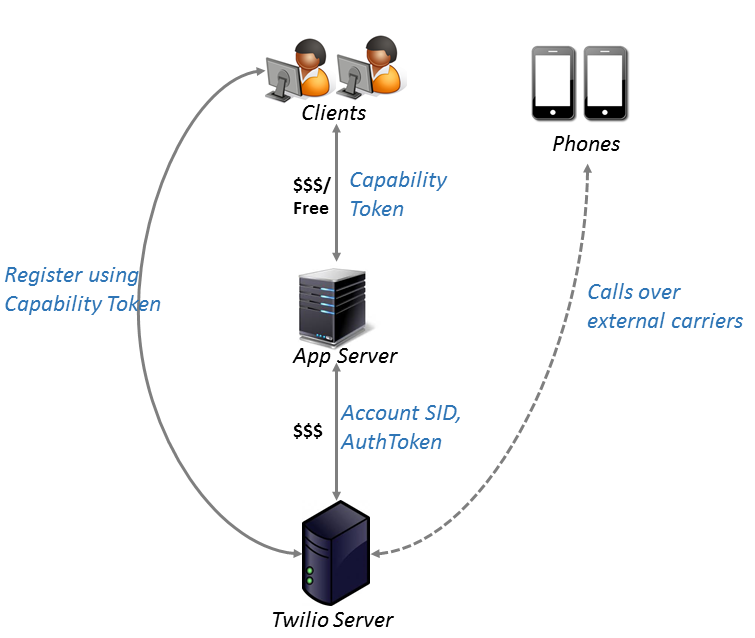
\includegraphics[width=0.45\textwidth]{figs/Ecosystem.png}
  %Mazu_frame_new.png}
\caption{Twilio Ecosystem}
\label{fig:ecosystem}
\end{figure}     